\chapter{Csontok}

\keywords{testi fájdalom meditáció közben}

\noindent Még ha jó testtartással is ülünk, előbb vagy utóbb valami
valahol fájni fog. A jó testtartás minimalizálja a szükségtelen
kényelmetlenséget, de nem tudja teljesen megszüntetni. A fájdalom és
kényelmetlenség ténye együtt jár azzal, hogy van testünk, de nem azért
meditálunk, hogy kínozzuk magunkat, és ügyelhetünk arra, hogy elkerüljük
a sérülést.

A testi fájdalmat vizsgálhatjuk, mint a meditáció tárgyát, figyelhetünk
a test egy másik területére, ahol nincs fájdalom, vagy változtathatunk a
testtartásunkon.

Ha a megszokott reakciónk a fájdalomra szorongás, ellenszenv és
nyugtalanság, akkor a vizsgálódás hasznosnak bizonyulhat. Emlékezz, hogy
a szándékod az, hogy jót akarsz magadnak. Ezután vizsgáld, figyeld meg a
fájdalmat, hogyan mozog a testben, hogyan keletkezik és múlik el
hullámokban. `Ki az, aki szenved? Változik ez? Hol van a tudatosság, ami
ezt tudja?' Ez megváltoztatja miként észleljük a fájdalmat. A
tapasztalatunk megváltozik, egy vészhelyzetből amit azonnal meg kell
oldanunk, egy jelzéssé, amit választásunk szerint félre tehetünk egy
időre.

\enlargethispage*{\baselineskip}

Lehet, hogy a fájdalom nem jelent sérülést, hasonlóan a
kényelmetlenséghez, amit akkor érzünk, mikor végig kell ülnünk egy
hosszú utat a buszon. A figyelmünket tarthatjuk a test egy
másik, fájdalom nélküli részén, vagy módszeresen végig vezethetjük a
test különböző részein, megfigyelve a helyet, ahol nincs fájdalom, és
meditációnkat az ott tapasztalható érzetek szemléletével folytatjuk.

\clearpage
\null\thispagestyle{empty}%
\photoFullBleed{standing.jpg}%
\illustration{Álló Meditáció Testtartás}%
\label{illus-standing-meditation}%
\clearpage

Egy érdekes gyakorlat pontosan meghatározni, hol húzódnak a fájdalmas
terület határai. Éles ez a határ, vagy határozatlan? Rögzítve marad,
vagy fokozatosan más irányba tolódik? Az ilyen vizsgálat közben
megismerjük a fájdalom keletkező és elmúló természetét. Ezután már nem
olyan nagy ügy. Nem kell ellenszenvvel reagálnunk rá, tudunk hagyni némi
szabad teret a kellemetlen érzeteknek, hogy hadd legyenek.

Amikor eldöntöd, hogy ideje megmozdulni, mielőtt mozdulnál, állj meg egy
pillanatra és határozd meg tisztán a szándékot: `A testem iránti
együttérzésből mozdulok. Megváltoztatom a testtartásom, mert azt
kívánom, hogy a testem jól érezze magát és egészséges legyen.' Ezután
helyezd át a lábaidat, vagy válts testtartást. Ez egyben tartja az
éberség folytonosságát, és így nem az ellenszenvre vagy nyugtalanságra
reagálunk.

\keywords{a test vizsgálata, csontok, az 'én' képe}

Az ülő meditáció után, átválthatunk álló helyzetbe és hagyjuk az
ízületeket és izmokat ellazulni. Az álló helyzet több figyelmet igényel
az egyensúly megtartására, így a csontok, a test tartóelemei, jobban
érezhetőek.

A csontok a test központi, merev részeit képezik, amik meghatározzák az
alakját, mit képes és képtelen tenni. Csontok nélkül, a testünk egy
formátlan húspaca lenne. Csontokkal belső struktúrát nyer, ami megadja a
külső megjelenését, amit jól ismerünk. A tükörbe nézünk és azt
gondoljuk, `az én vagyok'.

\enlargethispage*{\baselineskip}

Mennyire vizsgáltuk meg a képet, mielőtt magunkat láttuk benne? Egy
rövid körvonal, kontraszt és szín máris kiváltja az `én' kép
megjelenését. Viszonylag állandó képünk van magunkról, a jelenben a több
évvel ezelőtti önmagunk képével azonosulunk. Mivel a változás lassú,
egyre kevesebb és kevesebb kulcsjellemzőre hagyatkozunk, hogy
felismerjük a tükörben látható képet.

Ha közelebb hajolunk és több jellemzőt látunk, vagy egy szokatlan
szögből mutat minket egy fotó, percekbe is beletelhet mire el tudjuk
dönteni, kit látunk. Mi határozza meg ez a képet? Ha a csontok egy kissé
mások lennének, a testnek más alakja lenne, és ez megváltoztatná nem
csak a külsőnket, de azt is, hogyan élünk.

\keywords{álló meditáció módszere, álló testtartás}

Állj egyenes, de rugalmas helyzetben, fordíts egy kis idő arra, hogy
megtaláld a kiegyensúlyozott tartást. Helyezd a lábfejeket
vállszélességbe, a térdeket engedd ellazulni és kissé behajlani, hogy
aktív részük legyen a test megtartásában. Ne zárd az ízületeket
egyenesre, az megfeszíti őket és a tartásod merevvé válik. Tartsd a
lábfejeket párhuzamosan, a lábujjakkal egyenesen előre mutatva. Forgasd
a csípőt előre a vízszintes vonal mentén, kissé behúzva az alsó részt. A
mozdulat ahhoz hasonlít, mintha egy vödröt fordítanál a felső nyílással
magad felé.

Döntsd a tested jobbra-balra kissé, és érezd ki a súlypontot. Fejleszd
azt az érzést, hogy te tartod a tested egyenesben, hogy ne dőljön el. A
test egyensúlyát jobb a sarkok felett tartani, mint előre dőlni és a
lábfejekre nehezkedni.

Tartsd a vállakat elég szélesen ahhoz, hogy megnyissák a mellkast a
könnyű légzéshez, de nem olyan szélesen, hogy feszültté váljanak. A
kézfejeket kényelmes például a combokon tartani, körülbelül azon a pont
fölött, ahol a zsebek vannak egy nadrágon.

Engedj magadnak rugalmasságot, végezz kis változtatásokat a tartáson,
ahogy az izmok hozzászoknak a helyzethez. Érezd ki az állásban az
egyensúlyt és figyeld a testet ahogy így tartod. A gravitáció lefelé
húzza, nyomást hoz létre a földön. Ha úgy jobb, behajthatod a kezeket a
has előtt, egyik tenyér a másikon, kényelmes helyzetben.

A szemek lehetnek nyitva vagy csukva. Ha álmos vagy jobb, ha nyitott
szemmel meditálsz, de tartsd a tekinteted a magad előtti pár méteren. Ha
egyenesen előre nézel, a figyelem iránya kifelé fordul, és a látótérben
megjelenő mozgás elvonja a figyelmed.

Ha becsukod a szemed, de erőltetettnek és fájdalmasnak érzed, figyeld
hova irányul a szem fókusza, amikor becsukod. Ha befelé húzódik, mintha
egy közeli tárgyra fókuszálna a szemhéjak mögött, a szemgolyó belső
oldalán lévő izmok erőlködnek, hogy befelé húzzák azokat, ez a
feszültség szárazságot és könnycsordulást is okozhat.

A hagyományos Buddha szobrokon a Buddha szeme kissé nyitva van. Ő éber,
nem alszik. Ne zárd a szemhéjakat szorosra, gyakorold ellazítani azokat;
engedd le őket nyomás nélkül. Bár a szemhéjak majdnem zárva vannak,
képzeld azt, hogy egy távoli dologra nézel, ez hagyja ellazulni az
izmokat. Egy keskeny sáv nyitva marad, némi fényt enged be. Az is segít,
ha megmasszírozod a belső oldali szemizmokat, a nagyujjak hegyével
körkörös mozgásban.

Vegyél egy lélegzetet, és figyeld, hogyan változik a testtartás légzés
közben. A rekeszizom behúzza a levegőt, a has előre mozdul, hogy helyet
adjon. A kulcscsontok megemelkednek, a mellkasi bordák kifelé nyílnak, a
test súlypontja kissé elmozdul.

Van valami, ami korlátozza a légzést? Ellenőrizd, hogy egyenesen állj, a
váll ne görnyedjen előre, ami gátolja a nyitott légzést.

Figyelj a fej egyensúlyára, találd meg a pozíciót, ahol a fej a saját
súlyával egyensúlyban ül a gerinc tetején, nem dől előre vagy húzódik
hátra. Irányítsd a tekintetet kissé lefelé, ahelyett, hogy egyenesen
előre néznél, mert a jövés-menés elvonja a figyelmed. Húzd be az állat
könnyedén, ne engedd előre kitolódni, irányítsd a tekintetek pár
méterrel magad elé a földre. Engedd a fejtetőt kicsit megemelkedni,
mintha tartaná az eget.

A fej pozíciója nagy mértékben befolyásolja a felsőtest tartását. Mivel
sokat ülünk székeken, kialakul a szokásunk, hogy a fejet előre tolva
tartjuk, ez megfeszíti az hátizmokat a gerinc mentén. Ezeket az izmokat
nem tudjuk tudatosan irányítani, de kipróbálhatod, milyen érzés kissé
visszahúzni a fejet. Érzed ki az egyensúlyt, ahol a hátizmok ellazulnak.

Kiegyensúlyozott testtartásban a csontok úgy ülnek egymáson, mint az
óvatosan egymásra helyezett kövek. Ha a gerinc jó tartásban van, a
gravitáció elég, hogy stabilan tartsa. Ez kellemes, könnyed egyensúlyt
teremt erőltetés nélkül.

\enlargethispage*{\baselineskip}

\keywords{testhez való hozzáállás, analitikus elme, jószándék}

Ha túl analitikus hozzáállással közelítjük meg a test vizsgálatát, ez
groteszk és sokkoló benyomásokat kavarhat fel. A magunk felé irányuló
jószándék tartja a meditációt egyensúlyban, és hozzáállásunk jótékony
marad.

Az intellektus működése során elvont fogalmakat épít, figyelmének
tárgyait elkülöníti az egésztől. Mikor a testet szemléli, lehet, hogy
annak különböző részeit absztrakt és élettelen tárgyként tekinti.
Emlékezzünk, hogy nem azért gyakoroljuk a meditációt, hogy a testtel
szemben ellenszenvet vagy elidegenedést keltsünk. A meditáció tiszta
megértése akkor működik jól, amikor a dolgokat a környezetükkel együtt
látja, semmi nem létezik elszigetelve, üres térben. A tudatosság
befogad, nem kizár, és ehhez a hozzáállásunk része kell legyen a nyitott
elfogadás és jószándék.

Ez a hozzáállásbeli különbség egy történetre emlékeztet Platónról és
Diogenészről. Platón éppen egy előadást tartott a diákjainak Athénban az
Akadémián, és az `ember' fogalmát úgy határozta meg, mint `tollatlan
kétlábúak'. Úgy esett, hogy Diogenész hallotta ezt, és mivel kedvelte az
gyakorlatias vicceket, behozott az Akadémiára egy kopasztott csirkét, és
feltartotta Platónnak, ``Íme! Hoztam neked egy embert.'' Úgy
gondolhatta, ez bemutatja, hogy bizonyos környezeti jellemzők hiányoznak
az ember túlságosan intellektuális meghatározásából, mint `tollatlan
kétlábú'.

A csoport az Akadémián kiegészítette a meghatározást, ``\ldots{} lapos
és széles körmökkel'', ami kielégítette az intellektuális tárgyalásukat,
de alighanem nem értették meg mire mutatott rá Diogenész.

\keywords{az egész testet megtapasztalni}

Figyeljük a testi érzeteket a belégzés és kilégzés közben. Irányítsd a
figyelmet befelé, éberen a benyomásra, hogy `a test ilyen'. Az elme nem
keres, nem a világban jár valahol. Nem igényel semmit, ami itt van az
elég. Éberséggel látjuk a testet, a lábfejeket, a lábakat, a hasat, a
mellkast, a karokat, a vállakat, a nyakat és a fejet. A test egy egészet
alkot, egy mozgó benyomás, érzékeny a lélegzetre.

\enlargethispage*{\baselineskip}

A testet így figyelni olyan, mint az esőt nézni. Nincs tennivaló, semmit
nem kell eldönteni. Az eső tovább folytatja a dolgát anélkül, hogy be
kellene avatkoznunk.

\clearpage

\vspace*{-\baselineskip}

\keywords{tiszta megértés, testre irányuló tudatosság, kioltani a haragot és vágyat}

A kártékony gondolatokat hasonlíthatjuk a szélben kavargó porhoz:
elhomályosítja a képet, nem látunk tőle semmit. A Buddha az éberség
hatását az elmére az esőhöz hasonlította, ahogy kimossa a port és
megtisztítja a levegőt. `Szüntesd meg az ilyen (kártékony) gondolatokat
és kérdéseket, ahogy az eső elmossa a port; A szívben elcsitulnak a
gondolatok, és helyben eléri a béke állapotát.'\footnote{\href{https://suttacentral.net/iti87/en/sujato}{Iti
  87}, A Látás Pusztítói}

Az elmére való éberség megállítja a kártékony jellemzők keletkezését,
fejleszti a jótékony jellemzőket, és így megtisztítja az elmét.
Észrevehetjük, hogy a világot nem egy rögzített módon tapasztaljuk: nem
elzárt, külső szemlélők vagyunk, mintha egy magunktól különálló világra
néznénk az ablakon át. Aktív szerepünk van a világ létrehozásában, amit
tapasztalunk, hiszen mi alkotjuk a benyomásait a figyelmünk módján
keresztül.

Amikor megalapoztad a tiszta megértést, és észreveszed, hogy az elme
egyre tisztább és stabilabb, vedd szemügyre, mi tette lehetővé ezt a
változást? Mit tettél? Mit \emph{nem} tettél? Nem kellett az érzéki
benyomásokat manipulálnod, vagy küzdened a gondolatokkal és érzelmekkel,
elegendő volt megváltoztatni a figyelem módját.

A figyelmünk módja hozza létre a referencia keretet, amiben
megtapasztaljuk az érzékek világát az észlelések és emlékek felfogásától
függően. Ez egy folyamat, ami egy bizonyos hozzáállást produkál, mint
egy, az időt feldolgozó függvényt, aminek eredményétől függően
felismerjük és értelmezzük önmagunkat a jelenben.

A figyelem változását arra használjuk, hogy ne tápláljuk tovább a
kártékony mentális tényezőket. A közvetlen tapasztalat szemszögéből,
annak megfelelően ahogy a dolgok vannak, végük szakad, a folytatáshoz
szükséges referencia pont nélkül.

Röviden úgy mondjuk, az elmére való éberség megtisztítja az elmét.

A testi tudatosság felé fordulunk, ami kioltja mind a haragot és vágyat.
Megváltoztatja a figyelmünk keretét, hasra esnek, mintha kihúztuk volna
alóluk a szőnyeget. A zsúfolt, kritikus és haragos gondolatok olyanok,
mint egy zajos műsor, vagy a hírek a tavalyi újságban. A témája már nem
érdekel minket, elvesztette a fontosságát, folyton csak körbe-körbe jár.
Tedd le a gondolkodást, mint egy fáradt túrázó a nehéz hátizsákot, és
maradj a test éber figyelmével.

Időnként elvonja valami a figyelmünket, vagy elkezdünk álmodozni; mindig
térj vissza a légzéshez és az álló helyzet testi érzeteihez. Ha állás
közben csak történetekről és belső fantáziákról gondolkodunk amíg meg
nem szólal a harang, azzal nem a belátás meditációt gyakoroljuk\ldots{}
hanem a buszra várakozást.

\keywords{emlékek mint én, történetek az énről}

Vizsgáld az elme állapotát mint tapasztalatot. A test észlelése és az
érzései azelőtt jelennek meg, hogy az `én' észlelését felépítenénk
belőle. Mire emlékszünk önmagunkról? Ha elfelejtjük, amikor tegnap
valaki gorombán ránk kiabált, vagy emlékezünk, amikor barátainkkal
töltöttük az időt, ez megváltoztatja miként tekintünk önmagunkra?

Ez a kapcsolat az emlékeink, érzéseink és elmeállapotunk között folyton
változik. A felfogott képek folyton változnak, az éber tudatosság
megismerésével a bizalmat abba helyezzük, ami ismeri ezt a változást.
Ezzel a változást egy nagyobb képen belül láthatjuk, és nem ragadunk meg
a félelemben. Önmagunk képét egy aktív folyamat hozza létre, részt
veszünk benne az emlékeinkkel, azok újra-értelmezésével. Felépítünk egy
történetet magunkról a múlt emlékeiből, és megválasztjuk mit teszünk
most.

\keywords{csontok, a test részei, megfelelni akarás, a külső megjelenés bírálata}

A testet és annak részeit szemlélve az elmét a változó benyomásokra
összpontosítjuk, mielőtt az `én' képe megjelenik. Ez a folyamat
lefegyverzi az önbírálatot, a félelmet és elvárásokat, amik mint a
mocsár lehúznak minket.

Figyeld az érzést, ahogy a csontok kapcsolódnak egymáshoz az
ízületeknél. Megjelenik egy belső struktúra érzete, a struktúra ami a
testet belülről tartja. Merev darabok, egyik vég a másikhoz kapcsolódik,
egymásra rakva egyre magasabbra. A lábakban érezzük a merev csontokat,
ahogy tartják a testünket. Az érzés a gravitációról és nyomásról
árulkodik. A csípő csont a lábakon nyugszik, a felső test ehhez
kapcsolva mozog. A mellkas bordái szétnyílnak és összehúzódnak a
légzéssel. A gerinc ív alakban tartja a súlyt. A fej ott ül a gerinc
tetején. A koponya csontjai megfeszítik az arcbőrt.

A testünk darabokból áll. Darabokból, amik egyes helyeken merevek, más
helyeken puhák és rugalmasak. Ezek együttállása adja meg a formáját.
Amikor egy személyre nézünk, nem látunk mást, mint a hajat a fejen, a
szőrt a testen, körmöket, fogakat és bőrt. Ebből építjük a személyt --
elég a másodperc törtrészéig rápillantanunk, majd felismerve a
körvonalat vagy egy tipikus jellemzőt, és azt gondoljuk, `Ez én vagyok.
Jól nézek ki?'

\clearpage
\figurepagelayout

\begin{figure}[h]
\caption{Az Én Tapasztalata és Illúziója}\label{fig-illusion-of-self}

\centering

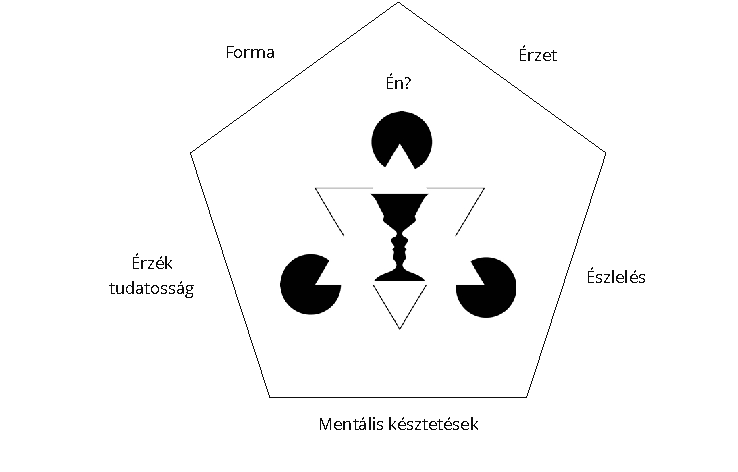
\includegraphics[width=80mm]{./manuscript/tex/diagrams/khandhas-self-illusion-hu.pdf}

\bigskip

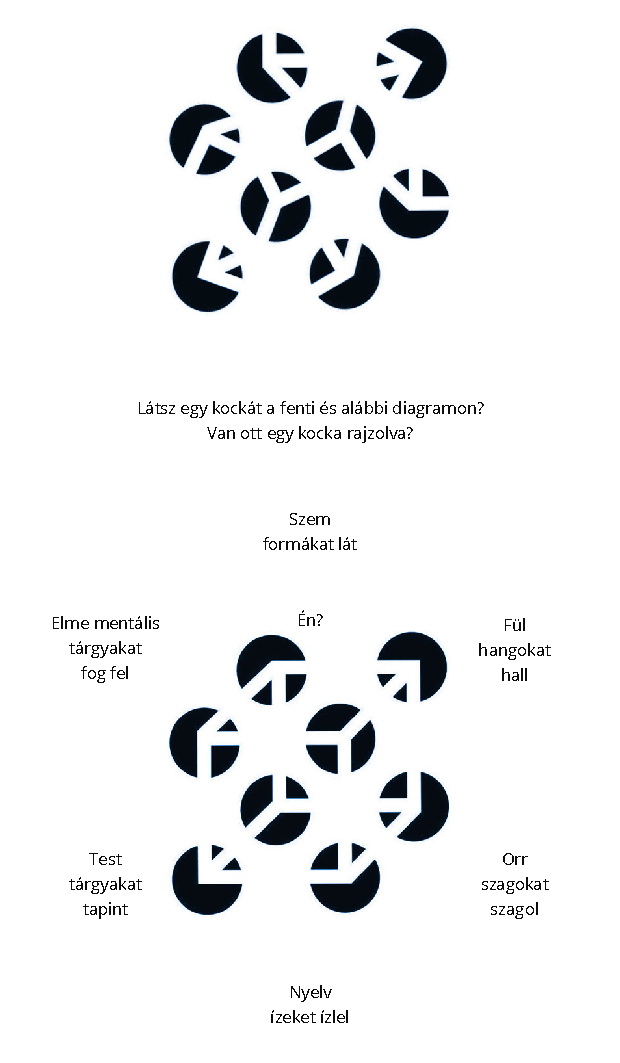
\includegraphics[width=80mm]{./manuscript/tex/diagrams/senses-self-illusion-hu.pdf}

\bigskip

\begin{minipage}{0.85\linewidth}
\centering\footnotesize
Tapasztalunk egy `én'-t, aminek nincs lényegi valósága azon a tapasztalaton kívül.
Ahogy fent látható, a kondicionált elvárások kitöltő alakokat hoznak létre
amit \emph{tapasztalunk}, de nincsenek ott.
A Kanizsa Háromszög, Rubin Váza és Szubjektív Necker Kocka az illúzió-kontúrok példái.
\end{minipage}

\end{figure}

\vfill\null
\clearpage
\normalpagelayout

Egyes helyzetekben láthatjuk a fokozatos felismerést az általánostól az
egyéniig, például amikor valakit látunk a ködben sétálni. Először
észrevesszük, hogy ez egy `személy' alakja, azután azt, hogy férfi vagy
nő. Lehet, hogy valaki akit ismerünk? Végül egy részlet kiváltja egy
barátunk felismerését és eszünkbe jut a neve. Mindez az észlelés
képeinek világában játszódik le.

Szokásunk, hogy a saját testünket, és másokét, egy töretlen egységként
látjuk, egyetlen dologként. Ebből a nézőpontból kialakul a megrögzött
gondolat, hogy van egy ideális formája és állapota. Elvárjuk, hogy a
testnek legyen bizonyos formája, magas vagy alacsony, és a további
jellemzői.

Ezek világi bírálatok, képek amit a kultúra amiben felnőttünk alakított
ki bennünk. Az egyik kultúra a vékony, a másik a telt testet tekinti
ideálisnak, és ezek a kulturális ideálok is változnak egyik generációról
a másikra. A hirdetések és a média üzenetei megerősítik ezeket az
elvárásokat és gondolkodás nélkül hiszünk bennük. Amikor közelebbről
szemügyre vesszük, azt látjuk, hogy ezek egy görbe tükör torzított
képei, nem egyeznek a valósággal.

Lehet, hogy mi sokat gondolunk arra, hogy mások mit gondolnak rólunk, de
\emph{mi magunk} mennyit törődünk mások küllemével? Ha magamat figyelem,
nem foglalkozok sokat más emberek kinézetével. De én zavarban tudom
érezni magam, és azt képzelem \emph{ők} biztos \emph{rólam}
gondolkodnak. Mikor valójában, annyit gondolnak rám, mint én rájuk --
alig, ha egyáltalán. A saját életükkel vannak elfoglalva, mint ahogy én
is az enyémmel.

\clearpage

Az önbírálatunk nyomása mellett, elképzeljük mások hogyan bírálnak
minket. Mivel nem tudhatjuk és nem irányíthatjuk mit gondolnak, az elme
belső párbeszédével megpróbáljuk megteremteni ezt a tudást és
irányítást, ami illúzió marad. Amikor lejátsszuk ezeket a belső
párbeszédeket, élvezzük ezt a megfoghatatlan irányítást. Viszont
lemaradunk arról a szabadságról, ami az irányítás igényének
elengedéséből születik.

\keywords{a test részeinek éntelen jellege}

Megfigyelhetjük az aggodalom feltételektől függő természetét, amikor a
test egyes részei elválnak. Sokat foglalkoztathat minket a hajunk
például, de csak addig, amíg a fejünkön van. Amikor a fodrász levágja,
nem törődünk a padlón összegyűlt hajkupaccal. Hasonló módon, mikor a
körmünket vágjuk, mikor van az a pont, amikor már nem `én' és `enyém'?

Így vizsgáljuk a testet, mint ami darabokból áll össze, és látjuk, hogy
a test nem egy bontatlan egység. Darabokból és részekből áll, amiknek
megvan a maguk természete, és aszerint viselkednek. Nem hallgatnak sem a
mi véleményünkre, sem a másokéra. Csontok, bőr, haj, fogak és körmök:
olyanok amilyenek, a saját természetüknek megfelelően.

A testünk egy áldás. Nem azért gyakoroljuk a meditációt, hogy
ellenszenvet keltsünk felé. Az egészség egy áldás, támogat minket
mindenben, amit teszünk. A Buddha az egészséget a legnagyobb kincsnek
nevezte.

\keywords{történetek mint álmok, testre irányuló tudatosság, szürke és élettelen állapotok, hála érzet}

Figyeljük a légzést, a test részeit, a jelen tapasztalatunkat. Azt
találjuk, hogy nem hordozzák magukkal az `én' és `enyém' történeteit.
Mivel mi hozzuk létre ezeket a történeteket, meg is tudjuk állítani
őket, nem vagyunk hozzájuk láncolva. A jelenségek függő kapcsolatokon
keresztül létre jönnek, a kapcsolat felbomlásával megszűnnek. Ez minden
ami történik.

A testre irányuló tudatosság enged a kívánságok szorításán és rávezet
arra, hogy szerencsések vagyunk, hogy itt lehetünk. Ehhez a figyelemhez
mindig vissza tudunk térni, egy belégzés és kilégzés elég ahhoz, hogy
emlékezzünk a keletkezésre és elmúlására. A kétségek olyanná válnak,
mint a sztorik egy régi újságban. A múlt szálait nehéz követni és
fáradtságos kibogozni, mintha valaki más álmait kellene értelmeznünk.

Ami valós, az mindig itt van a jelen tapasztalatunkban. Nem az válik
fontossá, hogy kik vagy mik vagyunk a történetben, hanem az, hogy a
figyelmünket a jelennek tudjuk szentelni.

\enlargethispage*{\baselineskip}

A tiszta szándéknak fontos szerepe van. Amikor nincs tisztán
elhatározott szándékunk, egyszerűen csak sodródunk. Nem kifejezetten
zavar minket, hogy itt vagyunk, de az elme szürke és élettelen, egy
jövőbeli időre vár, és addig próbál elbújni és láthatatlanná válni. Az
eredmény, hogy valóban szürkévé és láthatatlanná válunk. Semmi rossz nem
történik, de nincs semmi fény és öröm abban, hogy itt vagyunk.

Nem állunk meg elég gyakran, hogy észrevegyük mikor boldogok és
nyugodtak vagyunk. Amikor az elme tiszta és csendes, természetes módon
hálás azért ami itt van, és az áldásokért amit életünkben kaptunk.

A hálát nem lehet akarattal erőltetni. A gyakorlásban nem létrehozunk
valamit, hanem tiszta szándékkal felismerjük azt ami itt van. Nem erő
vagy képesség kérdése, ezek időhöz és körülményhez kötöttek. Az
elhatározás, a befelé irányuló felismerő figyelem nem egy adott
körülményhez kötött. Az eredmény a helyes szemlélet, amiben látjuk a
dolgok megfelelő helyét, és hogy mit kell azokkal tenni -- vagy csak
megállni, figyelni és lélegezni.
